
%*******************************************************************************
%*********************************** Second Chapter ***************************
%*******************************************************************************
%!TEX root = 0.main.tex

\section{Other samplings and other Discrete Laplacians}

\subsection{Heat Kernel Graph Laplacian on the Equiangular Sampling}
Presenting the results, showing how worse they are compared to HEALPix. Discuss why.
\subsection{Other Discrete Laplacians}
Present all the other ways of approximating the Laplace-Beltrami operator you found: graphs, Laplace de Rham, FEM
\subsection{Using the Finite Element Method to approximate the Laplace-Beltrami operator on a manifold}
\subsubsection{Galerkin Method and Finite Element Method}
General introduction to the FEM: definitions, weak formulation, functional spaces, Galerkin method, linear FEM.
\subsubsection{The eigenvalue problem on a manifold}
Weak formulation of the eigenvalue problem on the sphere, generalized eigenvalue problem, lumping of the mass matrix, discussion on the solvers
\subsection{Results}
\begin{figure}[h]
	\label{fig:HeatKernelGraphLaplacianHealpix}
	\caption{Heat Kernel Graph Laplacian on HEALPix}
	\centering
	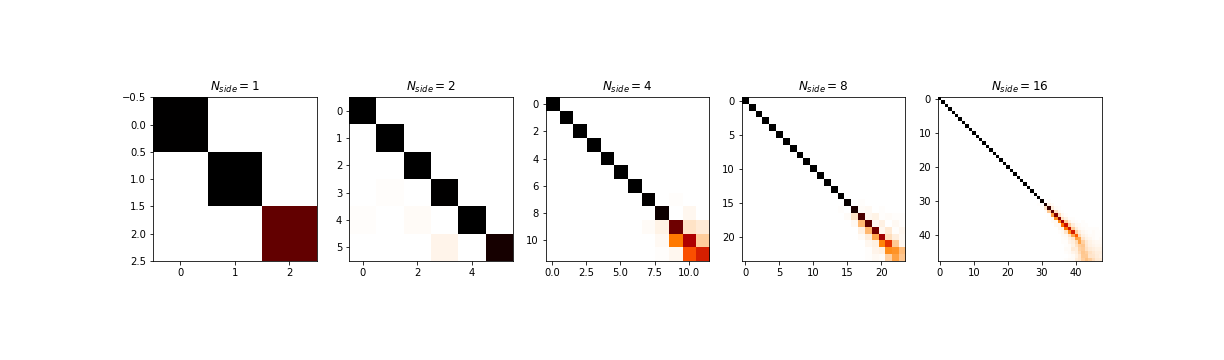
\includegraphics[width=0.9\textwidth]{../codes/02.HeatKernelGraphLaplacian/HEALPix/06_figures/optimal_thresholded.png}
	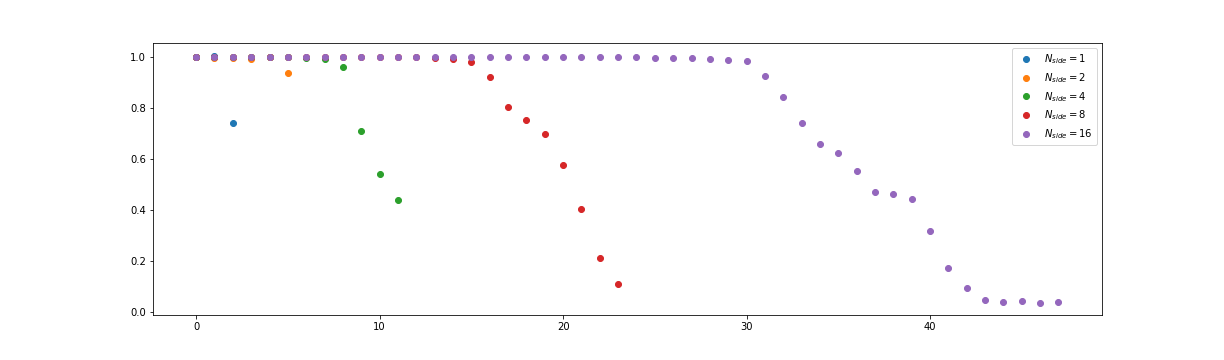
\includegraphics[width=0.9\textwidth]{../codes/02.HeatKernelGraphLaplacian/HEALPix/06_figures/optimal_thresholded_diagonal.png}	
\end{figure}

\begin{figure}[h]
	\label{fig:FEMHealpix}
	\caption{Linear FEM Laplacian on HEALPix}
	\centering
	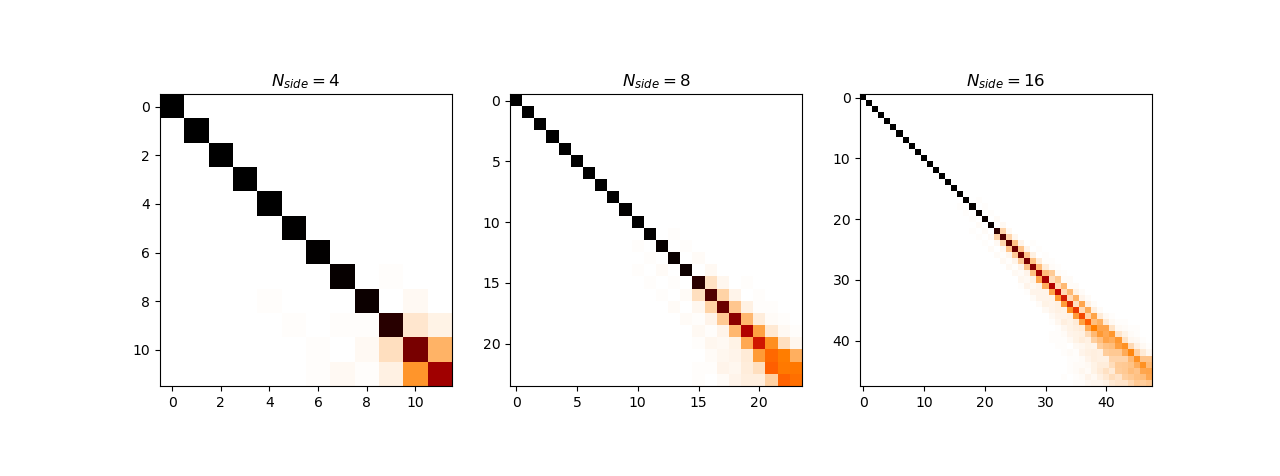
\includegraphics[width=0.9\textwidth]{../codes/03.FEM_laplacian/HEALPix/img/linearFEM.png}
	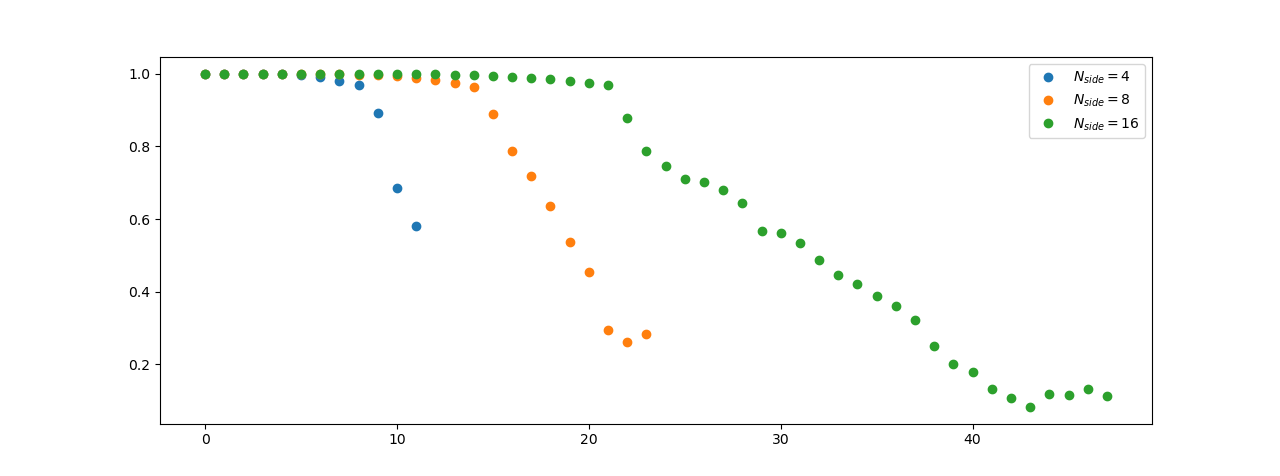
\includegraphics[width=0.9\textwidth]{../codes/03.FEM_laplacian/HEALPix/img/linearFEM_diagonal.png}	
	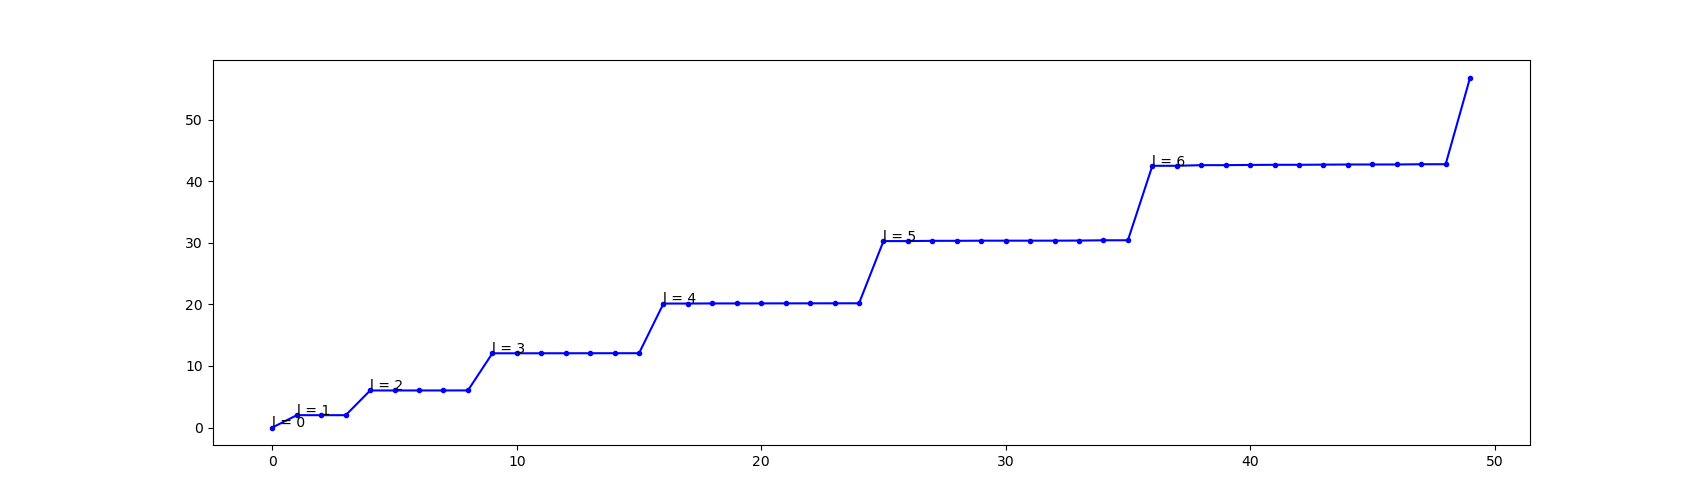
\includegraphics[width=0.9\textwidth]{../codes/03.FEM_laplacian/HEALPix/img/FEM_eigenvalues_16.png}	
	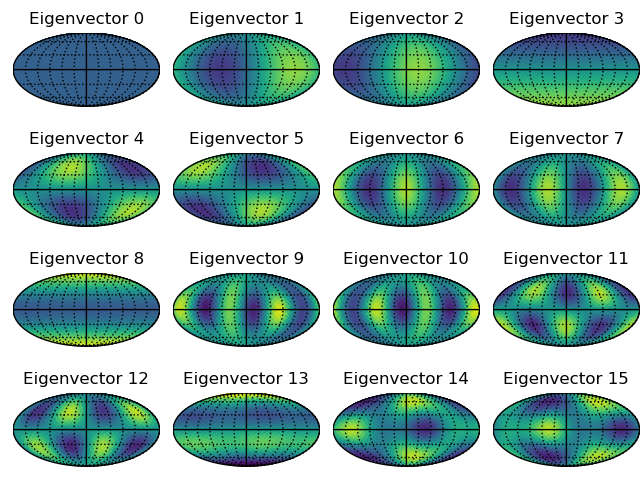
\includegraphics[width=0.7\textwidth]{../codes/03.FEM_laplacian/HEALPix/img/linear_FEM_8_eigenvectors.png}	
\end{figure}

\begin{figure}[h]
	\label{fig:HeatKernelGraphLaplacianEquiangular}
	\caption{Linear FEM Laplacian on equiangular sampling}
	\centering
	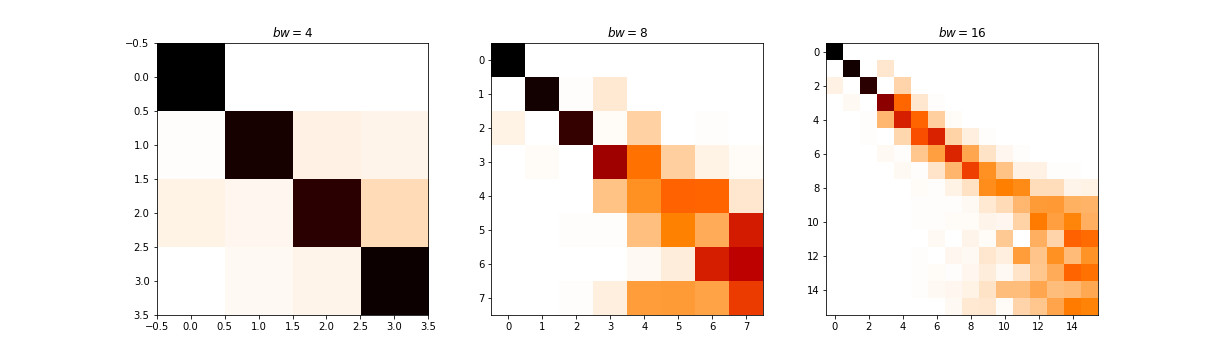
\includegraphics[width=0.9\textwidth]{../codes/02.HeatKernelGraphLaplacian/equiangular/equi_full.png}
	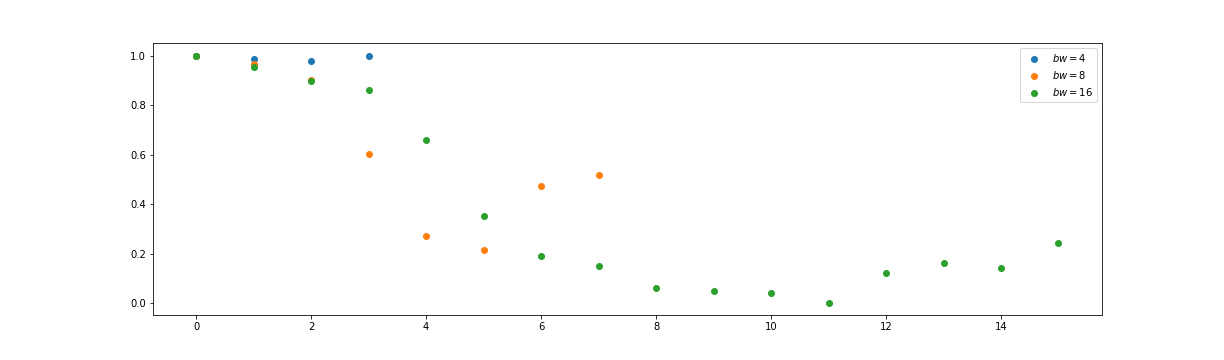
\includegraphics[width=0.9\textwidth]{../codes/02.HeatKernelGraphLaplacian/equiangular/equi_full_diagonal.png}	
	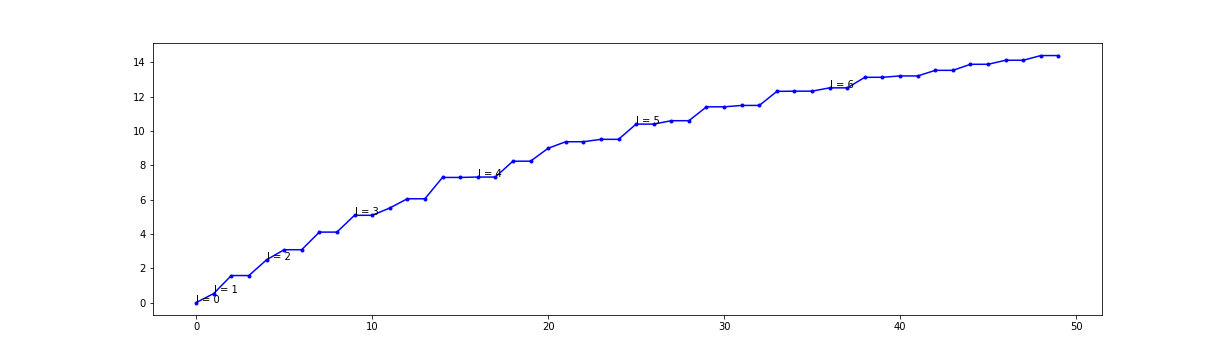
\includegraphics[width=0.9\textwidth]{../codes/02.HeatKernelGraphLaplacian/equiangular/equi_full_eigenvalues_16.png}	
\end{figure}

\begin{figure}[h]
	\label{fig:FEMequiangular}
	\caption{Linear FEM Laplacian on equiangular sampling}
	\centering
	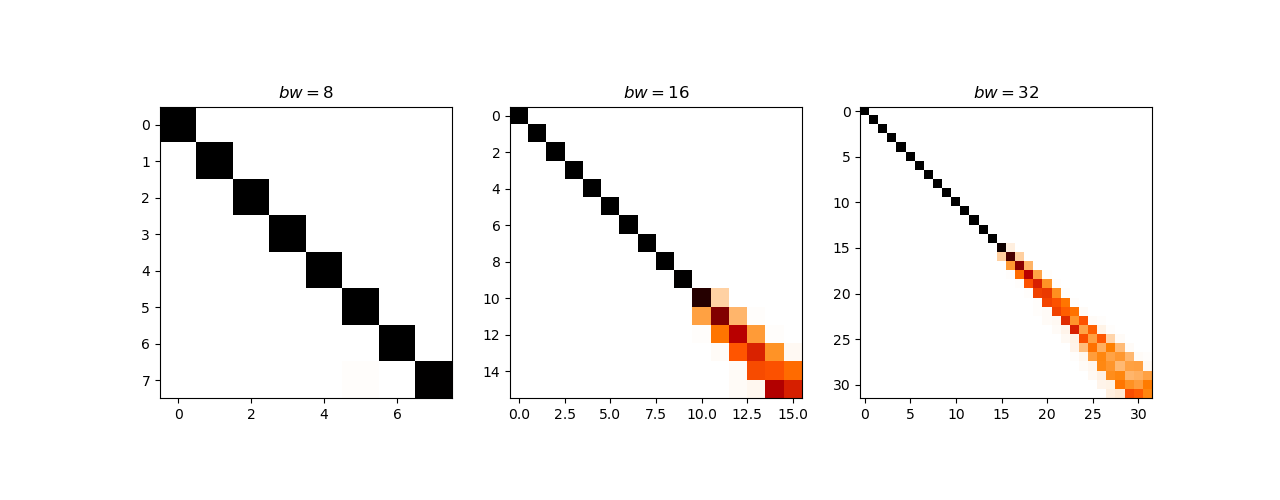
\includegraphics[width=0.9\textwidth]{../codes/03.FEM_laplacian/equiangular/normal/img/linearFEM.png}
	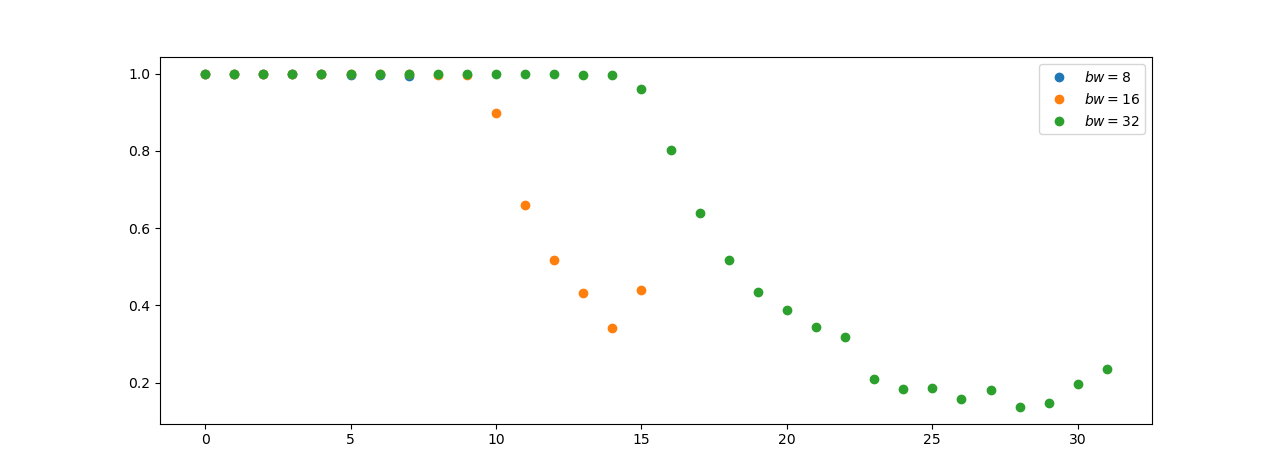
\includegraphics[width=0.9\textwidth]{../codes/03.FEM_laplacian/equiangular/normal/img/linearFEM_diagonal.png}	
	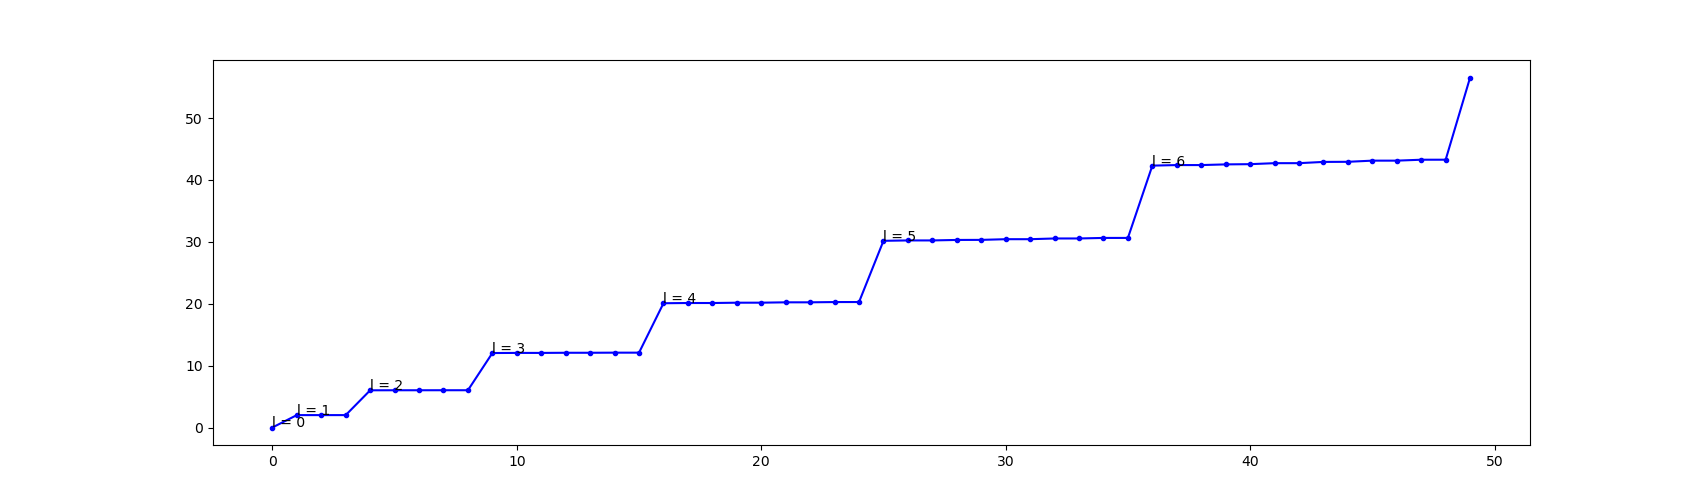
\includegraphics[width=0.9\textwidth]{../codes/03.FEM_laplacian/equiangular/normal/img/FEM_eigenvalues_16.png}	
\end{figure}

\begin{figure}[h]
	\label{fig:FEMequiangularLumped}
	\caption{Lumped Linear FEM Laplacian on equiangular sampling}
	\centering
	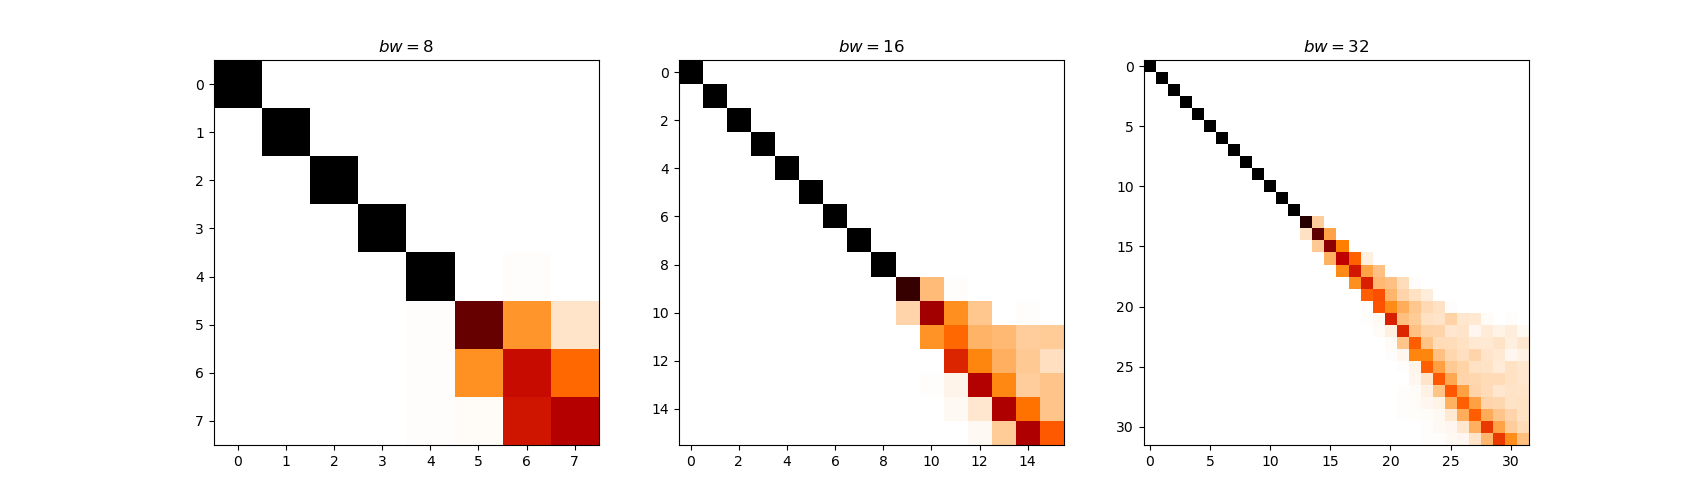
\includegraphics[width=0.9\textwidth]{../codes/03.FEM_laplacian/equiangular/mass_lumping/BL/img/linearFEM.png}
	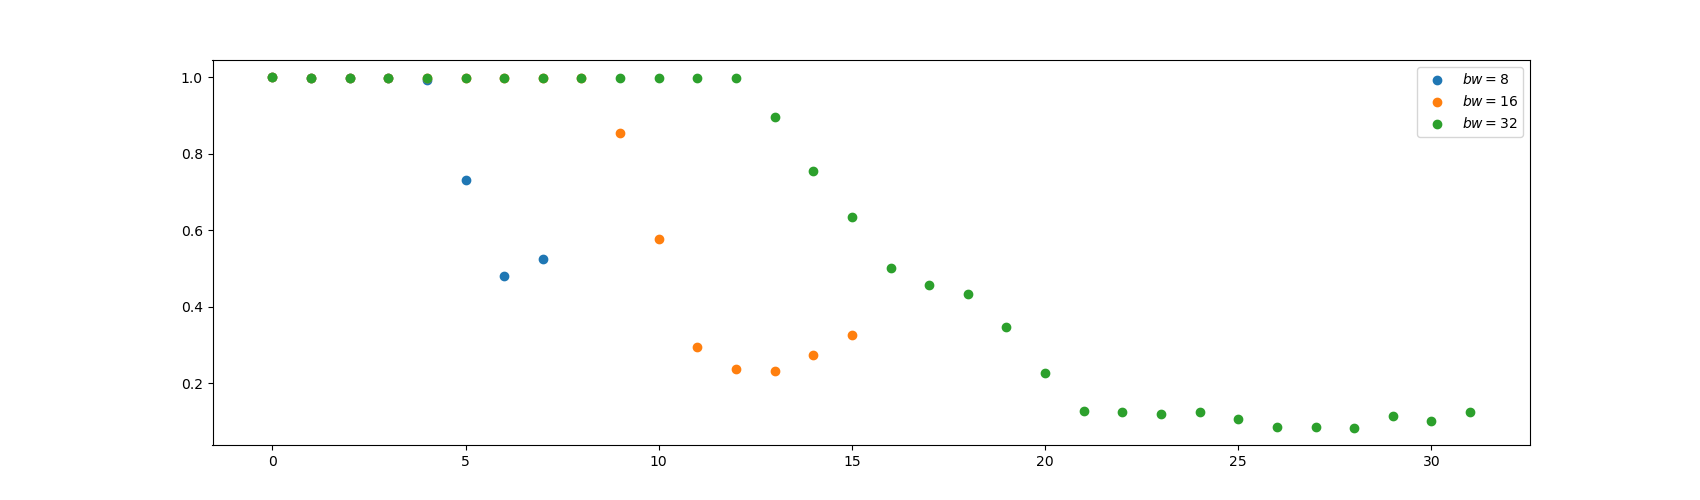
\includegraphics[width=0.9\textwidth]{../codes/03.FEM_laplacian/equiangular/mass_lumping/BL/img/linearFEM_diagonal.png}	
	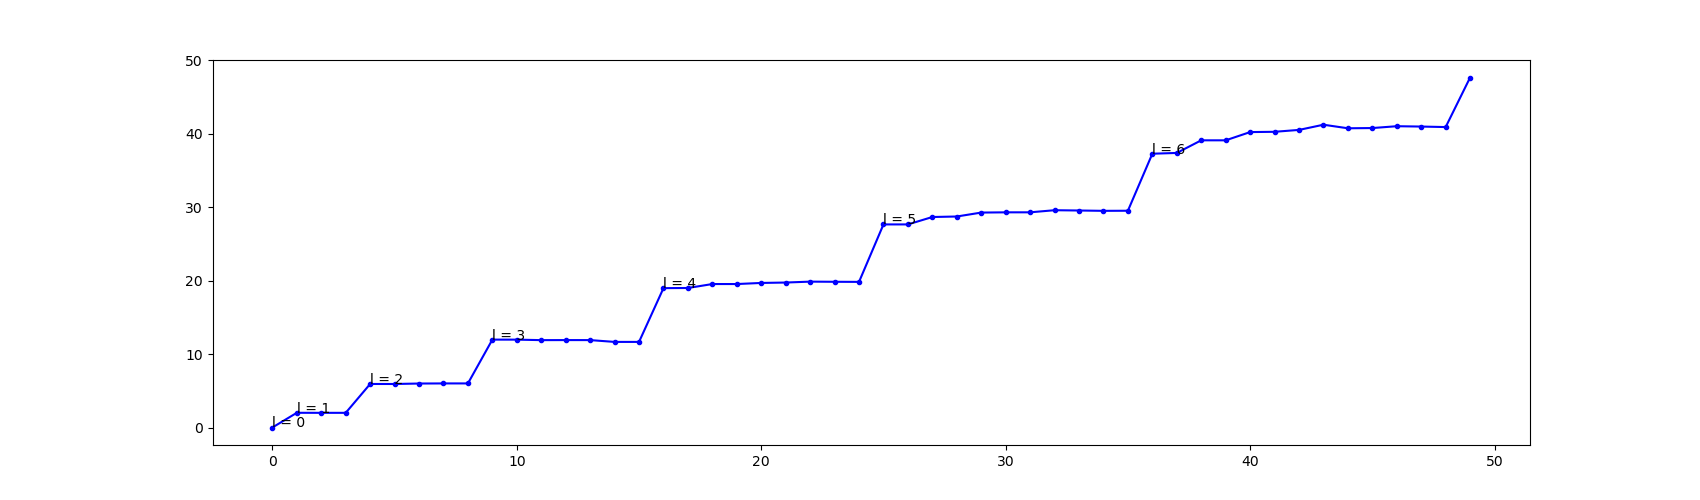
\includegraphics[width=0.9\textwidth]{../codes/03.FEM_laplacian/equiangular/mass_lumping/BL/img/FEM_eigenvalues_32.png}	
\end{figure}

\begin{figure}[h]
	\label{fig:symmetricFEMequiangularLumped}
	\caption{Symmetric Lumped Linear FEM Laplacian on equiangular sampling}
	\centering
	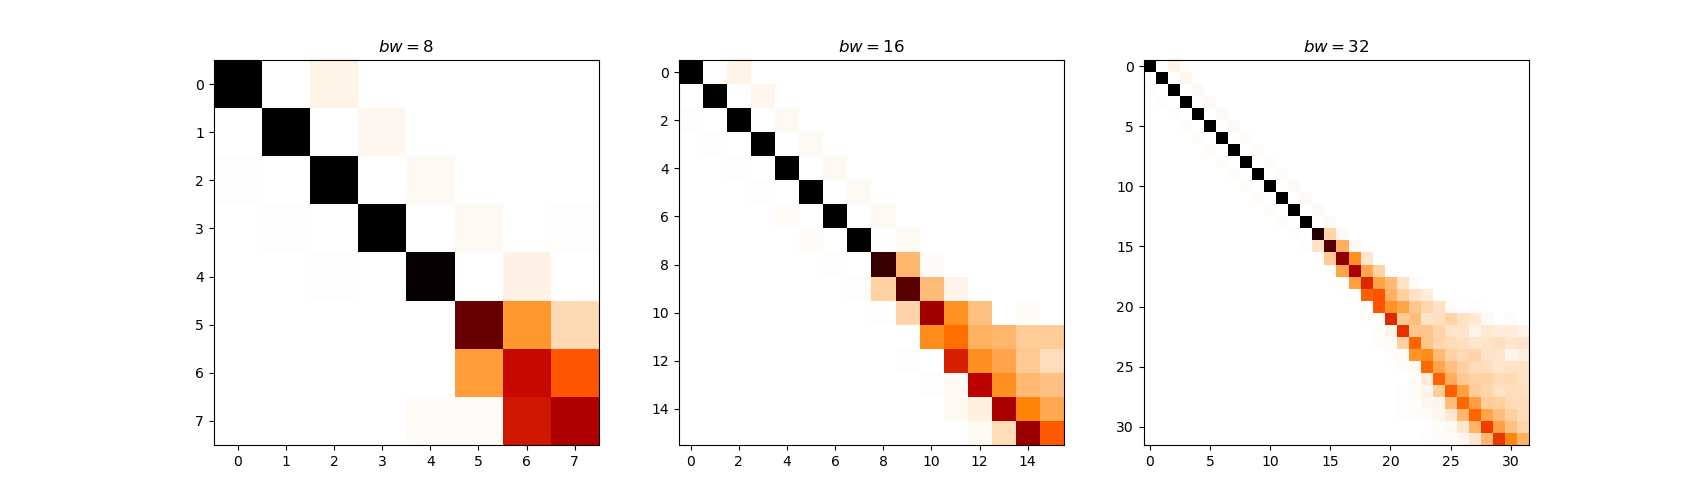
\includegraphics[width=0.9\textwidth]{../codes/03.FEM_laplacian/equiangular/mass_lumping/BLB/img/linearFEM.png}
	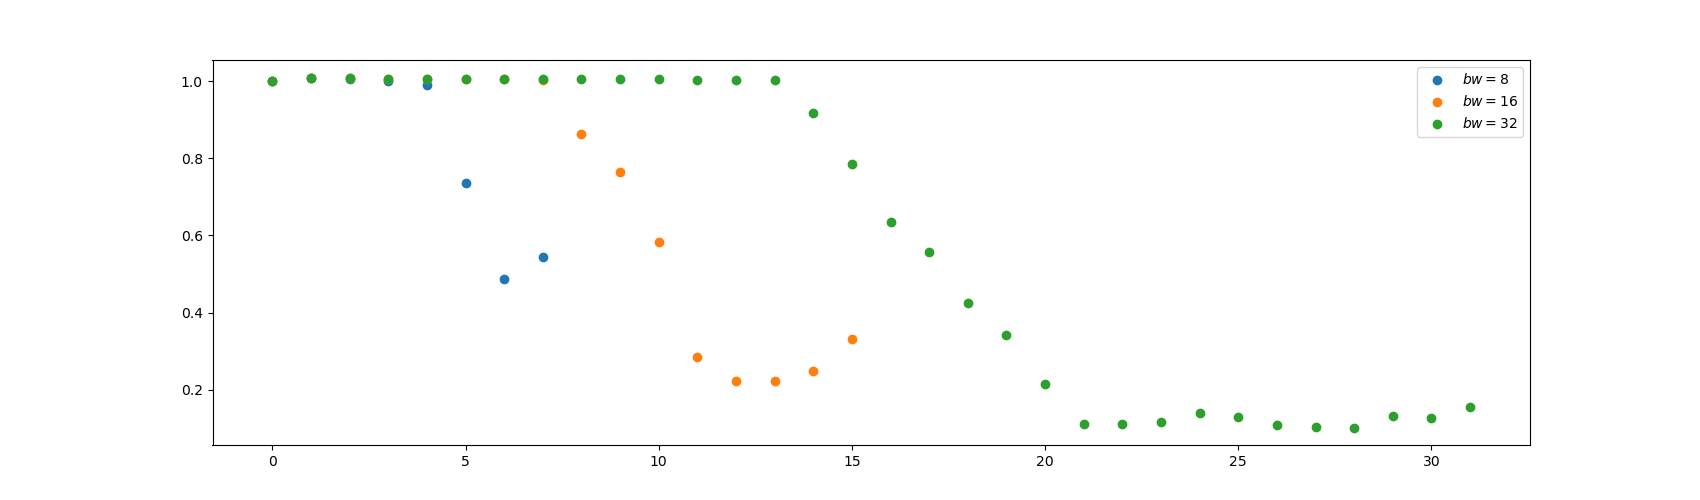
\includegraphics[width=0.9\textwidth]{../codes/03.FEM_laplacian/equiangular/mass_lumping/BLB/img/linearFEM_diagonal.png}	
	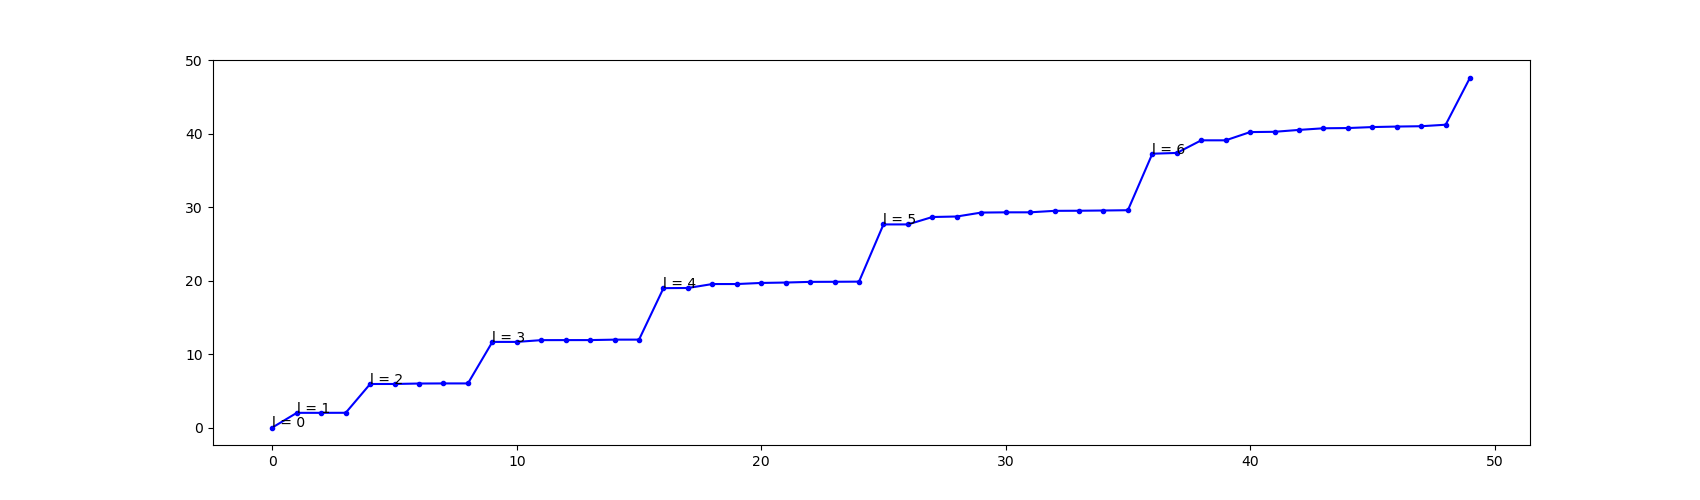
\includegraphics[width=0.9\textwidth]{../codes/03.FEM_laplacian/equiangular/mass_lumping/BLB/img/FEM_eigenvalues_32.png}	
\end{figure}